\section{Messung des Staudruckes}

Dieser Versuchsteil dient als Vorbereitung für die kommenden Versuche, um den am besten geeigneten Ort für die weiteren Messungen heraus zu finden. Dafür werden drei verschiedene Abstände vom Gebläseende gewählt, bei denen jeweils im Mittelpunkt und für 5 unterschiedlichen Abstände dessen gemessen wird. Da das System invariant ist unter Drehungen um die Mittelpunktachse des Gebläses werden der Einfachheit halber die Abstände vom Mittelpunkt nach oben gewählt.
\subsection{Messaufbau}

\begin{figure}
    \centering
    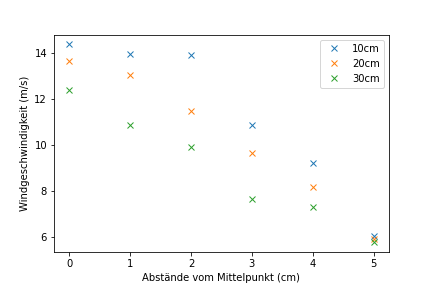
\includegraphics{Aeromechanik/Protokoll/fig/Aeromechanik Versuch 1.1.png}
    \caption{Windgeschwindigkeiten für drei verschiedene Abstände vom Gebläse}
    \label{fig:Aeromechanik Versuch 1.1}
\end{figure}

\section{Messung der Windgeschwindigkeit}
\subsection{Messaufbau}

\begin{figure}
    \centering
    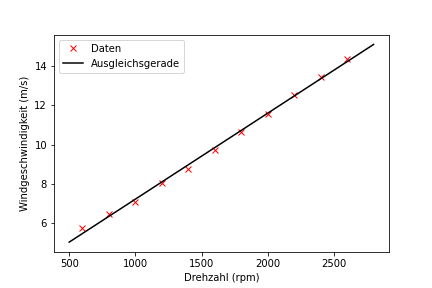
\includegraphics{Aeromechanik/Protokoll/fig/Aeromechanik Versuch 1.2.png}
    \caption{Windgeschwindigkeiten für verschiedene Drehzahlen}
    \label{fig:Aeromechanik Versuch 1.2}
\end{figure}